% Options for packages loaded elsewhere
\PassOptionsToPackage{unicode}{hyperref}
\PassOptionsToPackage{hyphens}{url}
\PassOptionsToPackage{dvipsnames,svgnames,x11names}{xcolor}
%
\documentclass[
  10pt,
  a4paper,
  DIV=11,
  oneside]{scrartcl}

\usepackage{amsmath,amssymb}
\usepackage{iftex}
\ifPDFTeX
  \usepackage[T1]{fontenc}
  \usepackage[utf8]{inputenc}
  \usepackage{textcomp} % provide euro and other symbols
\else % if luatex or xetex
  \usepackage{unicode-math}
  \defaultfontfeatures{Scale=MatchLowercase}
  \defaultfontfeatures[\rmfamily]{Ligatures=TeX,Scale=1}
\fi
\usepackage{lmodern}
\ifPDFTeX\else  
    % xetex/luatex font selection
    \setmainfont[]{Arial}
\fi
% Use upquote if available, for straight quotes in verbatim environments
\IfFileExists{upquote.sty}{\usepackage{upquote}}{}
\IfFileExists{microtype.sty}{% use microtype if available
  \usepackage[]{microtype}
  \UseMicrotypeSet[protrusion]{basicmath} % disable protrusion for tt fonts
}{}
\makeatletter
\@ifundefined{KOMAClassName}{% if non-KOMA class
  \IfFileExists{parskip.sty}{%
    \usepackage{parskip}
  }{% else
    \setlength{\parindent}{0pt}
    \setlength{\parskip}{6pt plus 2pt minus 1pt}}
}{% if KOMA class
  \KOMAoptions{parskip=half}}
\makeatother
\usepackage{xcolor}
\usepackage[top=30mm,left=20mm,heightrounded]{geometry}
\setlength{\emergencystretch}{3em} % prevent overfull lines
\setcounter{secnumdepth}{3}
% Make \paragraph and \subparagraph free-standing
\makeatletter
\ifx\paragraph\undefined\else
  \let\oldparagraph\paragraph
  \renewcommand{\paragraph}{
    \@ifstar
      \xxxParagraphStar
      \xxxParagraphNoStar
  }
  \newcommand{\xxxParagraphStar}[1]{\oldparagraph*{#1}\mbox{}}
  \newcommand{\xxxParagraphNoStar}[1]{\oldparagraph{#1}\mbox{}}
\fi
\ifx\subparagraph\undefined\else
  \let\oldsubparagraph\subparagraph
  \renewcommand{\subparagraph}{
    \@ifstar
      \xxxSubParagraphStar
      \xxxSubParagraphNoStar
  }
  \newcommand{\xxxSubParagraphStar}[1]{\oldsubparagraph*{#1}\mbox{}}
  \newcommand{\xxxSubParagraphNoStar}[1]{\oldsubparagraph{#1}\mbox{}}
\fi
\makeatother


\providecommand{\tightlist}{%
  \setlength{\itemsep}{0pt}\setlength{\parskip}{0pt}}\usepackage{longtable,booktabs,array}
\usepackage{calc} % for calculating minipage widths
% Correct order of tables after \paragraph or \subparagraph
\usepackage{etoolbox}
\makeatletter
\patchcmd\longtable{\par}{\if@noskipsec\mbox{}\fi\par}{}{}
\makeatother
% Allow footnotes in longtable head/foot
\IfFileExists{footnotehyper.sty}{\usepackage{footnotehyper}}{\usepackage{footnote}}
\makesavenoteenv{longtable}
\usepackage{graphicx}
\makeatletter
\newsavebox\pandoc@box
\newcommand*\pandocbounded[1]{% scales image to fit in text height/width
  \sbox\pandoc@box{#1}%
  \Gscale@div\@tempa{\textheight}{\dimexpr\ht\pandoc@box+\dp\pandoc@box\relax}%
  \Gscale@div\@tempb{\linewidth}{\wd\pandoc@box}%
  \ifdim\@tempb\p@<\@tempa\p@\let\@tempa\@tempb\fi% select the smaller of both
  \ifdim\@tempa\p@<\p@\scalebox{\@tempa}{\usebox\pandoc@box}%
  \else\usebox{\pandoc@box}%
  \fi%
}
% Set default figure placement to htbp
\def\fps@figure{htbp}
\makeatother
% definitions for citeproc citations
\NewDocumentCommand\citeproctext{}{}
\NewDocumentCommand\citeproc{mm}{%
  \begingroup\def\citeproctext{#2}\cite{#1}\endgroup}
\makeatletter
 % allow citations to break across lines
 \let\@cite@ofmt\@firstofone
 % avoid brackets around text for \cite:
 \def\@biblabel#1{}
 \def\@cite#1#2{{#1\if@tempswa , #2\fi}}
\makeatother
\newlength{\cslhangindent}
\setlength{\cslhangindent}{1.5em}
\newlength{\csllabelwidth}
\setlength{\csllabelwidth}{3em}
\newenvironment{CSLReferences}[2] % #1 hanging-indent, #2 entry-spacing
 {\begin{list}{}{%
  \setlength{\itemindent}{0pt}
  \setlength{\leftmargin}{0pt}
  \setlength{\parsep}{0pt}
  % turn on hanging indent if param 1 is 1
  \ifodd #1
   \setlength{\leftmargin}{\cslhangindent}
   \setlength{\itemindent}{-1\cslhangindent}
  \fi
  % set entry spacing
  \setlength{\itemsep}{#2\baselineskip}}}
 {\end{list}}
\usepackage{calc}
\newcommand{\CSLBlock}[1]{\hfill\break\parbox[t]{\linewidth}{\strut\ignorespaces#1\strut}}
\newcommand{\CSLLeftMargin}[1]{\parbox[t]{\csllabelwidth}{\strut#1\strut}}
\newcommand{\CSLRightInline}[1]{\parbox[t]{\linewidth - \csllabelwidth}{\strut#1\strut}}
\newcommand{\CSLIndent}[1]{\hspace{\cslhangindent}#1}

%% load packages
\usepackage{sectsty}
\usepackage{fontspec}
\usepackage{scrlayer-scrpage}
\usepackage{fontspec}

% Define title formatting

%% Set font sizes for sections and subsections
\sectionfont{\fontsize{11}{16}\selectfont\bfseries} % Arial 14pt bold
\subsectionfont{\fontsize{10}{14}\selectfont} % Arial 12pt

\lehead[test1]{\pagemark}
\cehead[]{}
\rehead[test 2]{\leftmark}
\lohead[{\fontsize{8}{10}\selectfont\upshape\textbf{Institut Sekundarstufe I}} \\
\fontsize{8}{10}\selectfont\upshape Fabrikstrasse 8, CH-3012 Bern \\
\fontsize{8}{10}\selectfont\upshape T +41 31 309 21 15, contactdesk@phbern.ch, www.phbern.ch
]{\rightmark}
\rohead[PHBern]{}
\KOMAoption{captions}{tableheading}
\makeatletter
\@ifpackageloaded{tcolorbox}{}{\usepackage[skins,breakable]{tcolorbox}}
\@ifpackageloaded{fontawesome5}{}{\usepackage{fontawesome5}}
\definecolor{quarto-callout-color}{HTML}{909090}
\definecolor{quarto-callout-note-color}{HTML}{0758E5}
\definecolor{quarto-callout-important-color}{HTML}{CC1914}
\definecolor{quarto-callout-warning-color}{HTML}{EB9113}
\definecolor{quarto-callout-tip-color}{HTML}{00A047}
\definecolor{quarto-callout-caution-color}{HTML}{FC5300}
\definecolor{quarto-callout-color-frame}{HTML}{acacac}
\definecolor{quarto-callout-note-color-frame}{HTML}{4582ec}
\definecolor{quarto-callout-important-color-frame}{HTML}{d9534f}
\definecolor{quarto-callout-warning-color-frame}{HTML}{f0ad4e}
\definecolor{quarto-callout-tip-color-frame}{HTML}{02b875}
\definecolor{quarto-callout-caution-color-frame}{HTML}{fd7e14}
\makeatother
\makeatletter
\@ifpackageloaded{caption}{}{\usepackage{caption}}
\AtBeginDocument{%
\ifdefined\contentsname
  \renewcommand*\contentsname{Inhaltsverzeichnis}
\else
  \newcommand\contentsname{Inhaltsverzeichnis}
\fi
\ifdefined\listfigurename
  \renewcommand*\listfigurename{Abbildungsverzeichnis}
\else
  \newcommand\listfigurename{Abbildungsverzeichnis}
\fi
\ifdefined\listtablename
  \renewcommand*\listtablename{Tabellenverzeichnis}
\else
  \newcommand\listtablename{Tabellenverzeichnis}
\fi
\ifdefined\figurename
  \renewcommand*\figurename{Abbildung}
\else
  \newcommand\figurename{Abbildung}
\fi
\ifdefined\tablename
  \renewcommand*\tablename{Tabelle}
\else
  \newcommand\tablename{Tabelle}
\fi
}
\@ifpackageloaded{float}{}{\usepackage{float}}
\floatstyle{ruled}
\@ifundefined{c@chapter}{\newfloat{codelisting}{h}{lop}}{\newfloat{codelisting}{h}{lop}[chapter]}
\floatname{codelisting}{Listing}
\newcommand*\listoflistings{\listof{codelisting}{Listingverzeichnis}}
\makeatother
\makeatletter
\makeatother
\makeatletter
\@ifpackageloaded{caption}{}{\usepackage{caption}}
\@ifpackageloaded{subcaption}{}{\usepackage{subcaption}}
\makeatother
\makeatletter
\@ifpackageloaded{sidenotes}{}{\usepackage{sidenotes}}
\@ifpackageloaded{marginnote}{}{\usepackage{marginnote}}
\makeatother

\ifLuaTeX
\usepackage[bidi=basic]{babel}
\else
\usepackage[bidi=default]{babel}
\fi
\babelprovide[main,import]{ngerman}
\ifPDFTeX
\else
\babelfont{rm}[]{Arial}
\fi
% get rid of language-specific shorthands (see #6817):
\let\LanguageShortHands\languageshorthands
\def\languageshorthands#1{}
\ifLuaTeX
  \usepackage[german]{selnolig} % disable illegal ligatures
\fi
\usepackage{bookmark}

\IfFileExists{xurl.sty}{\usepackage{xurl}}{} % add URL line breaks if available
\urlstyle{same} % disable monospaced font for URLs
\hypersetup{
  pdftitle={Mikroplanung Mathematik},
  pdfauthor={Richard Conrardy},
  pdflang={de},
  colorlinks=true,
  linkcolor={(3,1.5)},
  filecolor={Maroon},
  citecolor={Blue},
  urlcolor={Blue},
  pdfcreator={LaTeX via pandoc}}


\title{Mikroplanung Mathematik}
\usepackage{etoolbox}
\makeatletter
\providecommand{\subtitle}[1]{% add subtitle to \maketitle
  \apptocmd{\@title}{\par {\large #1 \par}}{}{}
}
\makeatother
\subtitle{Lernumgebungen entwickeln}
\author{Richard Conrardy}
\date{07.06.2024}

\begin{document}
\maketitle


\href{https://porta.phbern.ch/content/page/61fbb3277513396a43d9373a}{Porta-Mathematik}
\href{https://ilias.phbern.ch/goto_phbern_grp_2127034.html}{Materialraum}

\section{Blockkurs}

\begin{tcolorbox}[enhanced jigsaw, opacitybacktitle=0.6, titlerule=0mm, left=2mm, colbacktitle=quarto-callout-note-color!10!white, breakable, opacityback=0, bottomtitle=1mm, arc=.35mm, colframe=quarto-callout-note-color-frame, title=\textcolor{quarto-callout-note-color}{\faInfo}\hspace{0.5em}{Zielgruppe}, toptitle=1mm, rightrule=.15mm, colback=white, bottomrule=.15mm, toprule=.15mm, leftrule=.75mm, coltitle=black]

Dieser Kurs ist konzipiert für Studierende mit etwas Vorwissen im
Bereich der Entwicklung einer Lernumgebung und dem Wunsch mit
Kommilitonen dran zu arbeiten und dem Wunsch während der Entwicklung
Feedback von Kommilitonen oder Dozierenden zu erhalten.

\end{tcolorbox}

\begin{tcolorbox}[enhanced jigsaw, opacitybacktitle=0.6, titlerule=0mm, left=2mm, colbacktitle=quarto-callout-tip-color!10!white, breakable, opacityback=0, bottomtitle=1mm, arc=.35mm, colframe=quarto-callout-tip-color-frame, title=\textcolor{quarto-callout-tip-color}{\faLightbulb}\hspace{0.5em}{Flipped Classroom (Blockkurs)}, toptitle=1mm, rightrule=.15mm, colback=white, bottomrule=.15mm, toprule=.15mm, leftrule=.75mm, coltitle=black]

Diese Lerngelegenheit ist mit Flipped Classroom Methode konzipiert.

\begin{quote}
\begin{enumerate}
\def\labelenumi{\arabic{enumi}.}
\tightlist
\item
  move most information-transmission teaching out of class
\item
  use class time for learning activities that are active and social and
\item
  require students to complete pre- and/or post-class activities to
  fully benefit from in-class work.
\end{enumerate}

(Abeysekera \& Dawson, 2015, S. 3)
\end{quote}

\end{tcolorbox}

\section{SOL}

\begin{tcolorbox}[enhanced jigsaw, opacitybacktitle=0.6, titlerule=0mm, left=2mm, colbacktitle=quarto-callout-note-color!10!white, breakable, opacityback=0, bottomtitle=1mm, arc=.35mm, colframe=quarto-callout-note-color-frame, title=\textcolor{quarto-callout-note-color}{\faInfo}\hspace{0.5em}{Zielgruppe}, toptitle=1mm, rightrule=.15mm, colback=white, bottomrule=.15mm, toprule=.15mm, leftrule=.75mm, coltitle=black]

Dieser Kurs ist konzipiert für Studierende mit \emph{individuellen}
Bedürfnissen, damit sie sich in einer Sprechstunde eine
massgeschneiderte Unterstützung einer Fachperson abholen können.

SOL eignet sich somit besonders gut für Personen mit viel Vorwissen und
engem Terminkalender welche entweder kein Peerfeedback von Kommilitonen
brauchen oder es sich selbst organisieren.

\end{tcolorbox}

\begin{tcolorbox}[enhanced jigsaw, opacitybacktitle=0.6, titlerule=0mm, left=2mm, colbacktitle=quarto-callout-tip-color!10!white, breakable, opacityback=0, bottomtitle=1mm, arc=.35mm, colframe=quarto-callout-tip-color-frame, title=\textcolor{quarto-callout-tip-color}{\faLightbulb}\hspace{0.5em}{Selbstorganisiertes Lernen (SOL-Kurs)}, toptitle=1mm, rightrule=.15mm, colback=white, bottomrule=.15mm, toprule=.15mm, leftrule=.75mm, coltitle=black]

Dies ist eine selbstorganisierte Lerngelegenheit. Das heisst, die
Studierenden ``steuern ihr Lernhandeln jedoch weitgehend selber, indem
sie selbständig Lernschritte definieren, ausführen, regulieren und
beurteilen.'' (Hilbe \& Herzog, 2011, S. 8)

Dem Dozierenden ``kommt dabei die Aufgabe zu, geeignete
Rahmenbedingungen für das Gelingen des Lernprozesses zu schaffen,
Lernstrategien zu vermitteln und die Schülerinnen und Schüler bei
Schwierigkeiten zu unterstützen.'' (Hilbe \& Herzog, 2011, S. 8)

Kurz bedeutet dies, dass Sie stets Hilfe abholen können, sei es
inhaltlich, organisatorisch oder anderer Art.

\end{tcolorbox}

\section{Präsenzkurs}

\begin{tcolorbox}[enhanced jigsaw, opacitybacktitle=0.6, titlerule=0mm, left=2mm, colbacktitle=quarto-callout-note-color!10!white, breakable, opacityback=0, bottomtitle=1mm, arc=.35mm, colframe=quarto-callout-note-color-frame, title=\textcolor{quarto-callout-note-color}{\faInfo}\hspace{0.5em}{Zielgruppe}, toptitle=1mm, rightrule=.15mm, colback=white, bottomrule=.15mm, toprule=.15mm, leftrule=.75mm, coltitle=black]

Dieser Kurs arbeitet mit ihnen gemeinsam die Schritte der Entwicklung
einer Lernumgebung auf und eignet sich für Personen ohne Vorerfahrung
mit dem Bedürfnis nach mehr Theoriewissen.

Die Lernumgebung kann parallel in Hausarbeit erstellt werden.

\end{tcolorbox}

\begin{longtable}[]{@{}
  >{\centering\arraybackslash}p{(\linewidth - 6\tabcolsep) * \real{0.0706}}
  >{\raggedright\arraybackslash}p{(\linewidth - 6\tabcolsep) * \real{0.1529}}
  >{\centering\arraybackslash}p{(\linewidth - 6\tabcolsep) * \real{0.4235}}
  >{\centering\arraybackslash}p{(\linewidth - 6\tabcolsep) * \real{0.3529}}@{}}
\toprule\noalign{}
\begin{minipage}[b]{\linewidth}\centering
Teil
\end{minipage} & \begin{minipage}[b]{\linewidth}\raggedright
Thema
\end{minipage} & \begin{minipage}[b]{\linewidth}\centering
Vorbereitung
\end{minipage} & \begin{minipage}[b]{\linewidth}\centering
Slides
\end{minipage} \\
\midrule\noalign{}
\endhead
\bottomrule\noalign{}
\endlastfoot
1 & Lernziele & \href{}{Lernmodul} & \href{Slides_01.qmd}{Slides} \\
2 & Vorwissen & \href{}{Lernmodul} & \href{Slides_02.qmd}{Slides} \\
3 & Stoffauswahl & \href{}{Lernmodul} & \href{}{Slides} \\
4 & Sozialformen und Phasen & \href{}{Lernmodul} & \href{}{Slides} \\
5 & Aufgaben & & \href{}{Slides} \\
6 & Überleitung & & \href{}{Slides} \\
\end{longtable}

\section{Workload}\label{workload}

Sie veröffentlichen eine Lernumgebung von 2 bis 4 Lektionen unter einer
freien Lizenz (Vorschlag:
\href{https://creativecommons.org/licenses/by-sa/4.0/}{CC BY-SA 4.0})
und zitieren nach APA 7 (vgl. American Psychological Association, 2020).

Tragen Sie sich für bei der Themenauswahl in die
\href{https://phbern365.sharepoint.com/:x:/r/sites/IS1_Z_FachteamMathematik/_layouts/15/Doc2.aspx?action=edit&sourcedoc=\%7B6d7b7b77-e701-495c-a734-95aa8c684020\%7D&wdOrigin=TEAMS-MAGLEV.teamsSdk_ns.rwc&wdExp=TEAMS-TREATMENT&wdhostclicktime=1725374697781&web=1&CID=2f77316a-b428-4c26-ed85-c19100b5eb17}{Themenliste}
ein.

Erstellen und veröffentlichen Sie ihre Lernumgebung auf
\href{https://portfolio.switch.ch/}{Switchportolio}.

\begin{tcolorbox}[enhanced jigsaw, opacitybacktitle=0.6, titlerule=0mm, left=2mm, colbacktitle=quarto-callout-tip-color!10!white, breakable, opacityback=0, bottomtitle=1mm, arc=.35mm, colframe=quarto-callout-tip-color-frame, title=\textcolor{quarto-callout-tip-color}{\faLightbulb}\hspace{0.5em}{Digileb Knowledge Base}, toptitle=1mm, rightrule=.15mm, colback=white, bottomrule=.15mm, toprule=.15mm, leftrule=.75mm, coltitle=black]

Das Digileb hat eine
\href{https://digileb.phbern.ch/medien-gestalten-und-nutzen/medien-gestalten/switchportfolio-gestalten/}{eine
Einleitung zu Switchportfolio} und zu
\href{https://digileb.phbern.ch/didaktisches-design/kollaboratives-lernen-und-arbeiten/oer-herstellen/}{Open
Educational Resources} verfasst.

\end{tcolorbox}

Sie planen eine bis zwei Doppellektionen für eine niveaudurchmischte
Klasse und geben folgende Materialien ab:

\begin{itemize}
\tightlist
\item
  Einführender Lehrpersonenkommentar inkl. zwei Vertiefungen
  (Motivation, Wirksamkeit, Lernphasen oder Wissenserwerb)
\item
  Lernmaterialien, inkl Lektionsplanung
\end{itemize}

\begin{tcolorbox}[enhanced jigsaw, opacitybacktitle=0.6, titlerule=0mm, left=2mm, colbacktitle=quarto-callout-warning-color!10!white, breakable, opacityback=0, bottomtitle=1mm, arc=.35mm, colframe=quarto-callout-warning-color-frame, title=\textcolor{quarto-callout-warning-color}{\faExclamationTriangle}\hspace{0.5em}{Warnung}, toptitle=1mm, rightrule=.15mm, colback=white, bottomrule=.15mm, toprule=.15mm, leftrule=.75mm, coltitle=black]

Die Lerngelegenheit kann abgeschlossen werden ohne Lehrpersonenkommentar
und Vertiefung. Der Fokus liegt auf den Lernmaterialien und den
dazugehörigen Methoden, Techniken und Medien. Die Auflistung ist als
Hinweis für den Leistungsnachweis zu verstehen. Informieren Sie sich auf
Bios über die offiziellen Kriterien und Inhalte.

\end{tcolorbox}

\begin{tcolorbox}[enhanced jigsaw, opacitybacktitle=0.6, titlerule=0mm, left=2mm, colbacktitle=quarto-callout-tip-color!10!white, breakable, opacityback=0, bottomtitle=1mm, arc=.35mm, colframe=quarto-callout-tip-color-frame, title=\textcolor{quarto-callout-tip-color}{\faLightbulb}\hspace{0.5em}{Schreibberatung}, toptitle=1mm, rightrule=.15mm, colback=white, bottomrule=.15mm, toprule=.15mm, leftrule=.75mm, coltitle=black]

Die Institut Sekundarstufe 1 bietet Ihnen eine Schreibberatung an. Falls
Sie wissenschaftlichen Schreiben, inkl. korrektes zitieren noch nicht
beherrschen, können Sie sich an \textbf{schreibberatung-is1@phbern.ch}
wenden.

\end{tcolorbox}

Sie begründen Ihre Planungen differenziert mathematikdidaktisch,
lernpsychologisch und mit Bezügen zu den Querschnittsthemen.

Folgende Beurteilungskriterien dienen Ihnen zur Orientierung:

\begin{itemize}
\tightlist
\item
  Die Lernumgebung enthält bedeutsame Inhalte, welche mit dem Lehrplan
  verbunden sind.
\item
  Die Lernumgebung ist fachlich-inhaltlich korrekt.
\item
  Die Lernumgebung ist zielgruppengerecht strukturiert.\\
\item
  In der Lernumgebung sind die Lernerwartungen zielgruppengerecht
  formuliert.
\item
  Der Lernprozess bei der Lernumgebung ist in sinnvolle Lernphasen
  gegliedert.
\item
  Die Lernumgebung enthält analoge wie digitale, fachliche,
  überfachliche und fächerübergreifende Teile mit entsprechenden
  sprachsensiblen Aufgaben.
\item
  Die Lernumgebung fördert partizipatives und individualisiertes Lernen.
\item
  In der Lernumgebung werden Sozialformen, Methoden, Medien und
  Materialien lernfördernd und abwechslungsreich eingesetzt.
\item
  Die Lernumgebung und zusätzlichen Erklärungen zeigen wie Lernprozesse
  fachwissenschaftlich, fachdidaktisch, allgemeindidaktisch,
  mediendidaktisch und lernpsychologisch gestaltet und begründet sind.
\end{itemize}

\subsection{Konventionen}\label{konventionen}

Grundsätzlich werden Notationen und Symbole nach ISO 80000-2:2009
übernommen. Dezimalzahlen werden mit Komma (``4,32'') geschrieben.
Koordinaten werden mit Strichpunkt (``4,1;2,7'') getrennt. Das
Geteiltzeichen ist ein Querstrich (``1/2'') oder Bruchstrich
(``\(\frac{1}{2}\)''). Der Doppelpunkt bezeichnet ein Verhältnis
(``4:3:2''). Das Multiplikationszeichen (falls vorhanden) ist ein Punkt
(``\(3\cdot 2\)''). Geogebrabefehle und
Tabellenkalkulationsprogrammbefehle sind auf Englisch.

Als Makroplanung orientieren wir uns an folgender Aufteilung:

\begin{figure*}

\begin{longtable}[]{@{}
  >{\raggedright\arraybackslash}p{(\linewidth - 14\tabcolsep) * \real{0.0829}}
  >{\raggedright\arraybackslash}p{(\linewidth - 14\tabcolsep) * \real{0.1710}}
  >{\raggedright\arraybackslash}p{(\linewidth - 14\tabcolsep) * \real{0.1295}}
  >{\raggedright\arraybackslash}p{(\linewidth - 14\tabcolsep) * \real{0.1503}}
  >{\raggedright\arraybackslash}p{(\linewidth - 14\tabcolsep) * \real{0.1036}}
  >{\raggedright\arraybackslash}p{(\linewidth - 14\tabcolsep) * \real{0.0725}}
  >{\raggedright\arraybackslash}p{(\linewidth - 14\tabcolsep) * \real{0.1140}}
  >{\raggedright\arraybackslash}p{(\linewidth - 14\tabcolsep) * \real{0.1451}}@{}}
\caption{Übersicht des Jahresablaufes}\tabularnewline
\toprule\noalign{}
\begin{minipage}[b]{\linewidth}\raggedright
\end{minipage} & \begin{minipage}[b]{\linewidth}\raggedright
Form
\end{minipage} & \begin{minipage}[b]{\linewidth}\raggedright
Zahl
\end{minipage} & \begin{minipage}[b]{\linewidth}\raggedright
Raum
\end{minipage} & \begin{minipage}[b]{\linewidth}\raggedright
Variable
\end{minipage} & \begin{minipage}[b]{\linewidth}\raggedright
Funktionen
\end{minipage} & \begin{minipage}[b]{\linewidth}\raggedright
Daten und Zufall
\end{minipage} & \begin{minipage}[b]{\linewidth}\raggedright
Erweiterung
\end{minipage} \\
\midrule\noalign{}
\endfirsthead
\toprule\noalign{}
\begin{minipage}[b]{\linewidth}\raggedright
\end{minipage} & \begin{minipage}[b]{\linewidth}\raggedright
Form
\end{minipage} & \begin{minipage}[b]{\linewidth}\raggedright
Zahl
\end{minipage} & \begin{minipage}[b]{\linewidth}\raggedright
Raum
\end{minipage} & \begin{minipage}[b]{\linewidth}\raggedright
Variable
\end{minipage} & \begin{minipage}[b]{\linewidth}\raggedright
Funktionen
\end{minipage} & \begin{minipage}[b]{\linewidth}\raggedright
Daten und Zufall
\end{minipage} & \begin{minipage}[b]{\linewidth}\raggedright
Erweiterung
\end{minipage} \\
\midrule\noalign{}
\endhead
\bottomrule\noalign{}
\endlastfoot
\begin{minipage}[t]{\linewidth}\raggedright
\begin{enumerate}
\def\labelenumi{\arabic{enumi}.}
\setcounter{enumi}{6}
\tightlist
\item
  Klasse HS
\end{enumerate}
\end{minipage} & Vierecke, Symmetrien & Primzahlen, kgV, ggT, &
Koordinatensystem, & Variablen, & Gleichungen & Diagramme, Prozente &
Potenzen \\
\begin{minipage}[t]{\linewidth}\raggedright
\begin{enumerate}
\def\labelenumi{\arabic{enumi}.}
\setcounter{enumi}{6}
\tightlist
\item
  Klasse FS
\end{enumerate}
\end{minipage} & Dreiecke, Kongruenzabbildungen & ganze Zahlen, Potenzen
& Volumen, Oberfläche, Kreis & Termumformung & Gleichungen & Ereignisse,
Prozent & Wurzeln, Proportionalität \\
\begin{minipage}[t]{\linewidth}\raggedright
\begin{enumerate}
\def\labelenumi{\arabic{enumi}.}
\setcounter{enumi}{7}
\tightlist
\item
  Klasse HS
\end{enumerate}
\end{minipage} & Thales

Pythagoras & Rationale Zahlen & Prismen,Kreissektoren & Termumformung &
Gleichungen & Kennwerte & wiss. Schreib. \\
\begin{minipage}[t]{\linewidth}\raggedright
\begin{enumerate}
\def\labelenumi{\arabic{enumi}.}
\setcounter{enumi}{7}
\tightlist
\item
  Klasse FS
\end{enumerate}
\end{minipage} & Pythagoras & Potenzen & Pyramiden & Gleichungen &
Funktionen & Mehrstuf. Exp. & Textaufg. \\
\begin{minipage}[t]{\linewidth}\raggedright
\begin{enumerate}
\def\labelenumi{\arabic{enumi}.}
\setcounter{enumi}{8}
\tightlist
\item
  Klasse HS
\end{enumerate}
\end{minipage} & Streckung, Strahlens. & Termumf. & Körper & Gleich. &
Lin. Funk. & Komb., Zinsen & Ungl. \\
\begin{minipage}[t]{\linewidth}\raggedright
\begin{enumerate}
\def\labelenumi{\arabic{enumi}.}
\setcounter{enumi}{8}
\tightlist
\item
  Klasse FS
\end{enumerate}
\end{minipage} & Ähnlichkeit & Termumf. & Kegel, Kugel &
Gleichungssysteme & Funkt. & Komb & \\
& & & & & & & \\
\end{longtable}

\end{figure*}%

Pro Jahr 39 (19+20) Schulwochen. Planung mit 36 (18+18) Wochen
-\textgreater{} Pro Feld 3 Wochen

\begin{figure}[H]

{\centering \pandocbounded{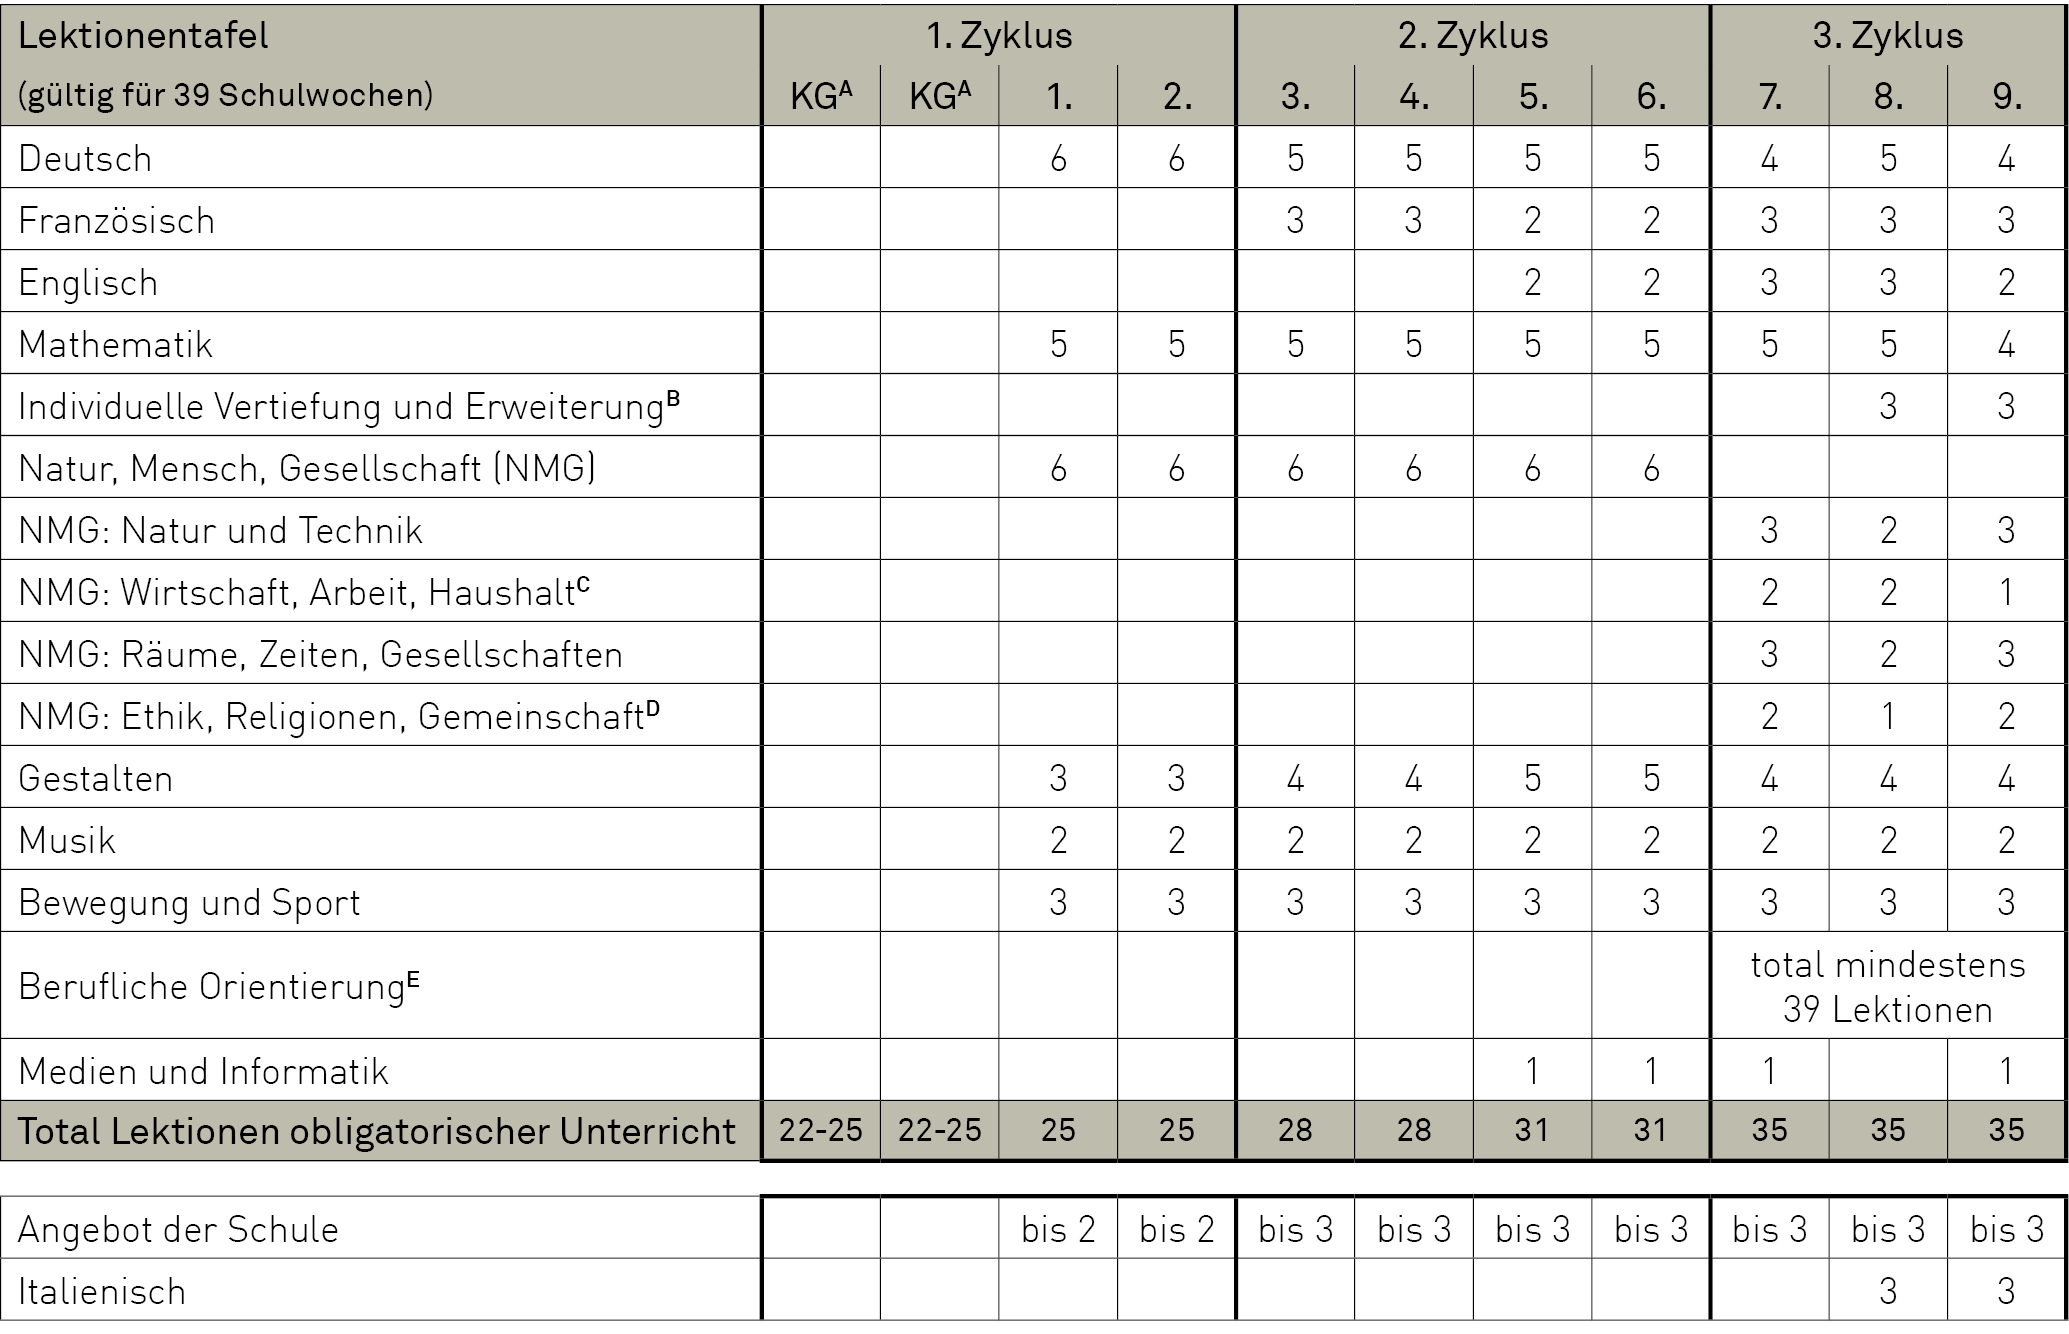
\includegraphics[keepaspectratio]{LG_mikroplanungmath_files/mediabag/ahb_kapitel_4.1.4.jpg}}

}

\caption{Lektionentafel}

\end{figure}%

\phantomsection\label{refs}
\begin{CSLReferences}{1}{0}
\bibitem[\citeproctext]{ref-abeysekera_motivation_2015}
Abeysekera, L., \& Dawson, P. (2015). Motivation and cognitive load in
the flipped classroom: definition, rationale and a call for research.
\emph{Higher Education Research \& Development}, \emph{34}(1), 1--14.
\url{https://doi.org/10.1080/07294360.2014.934336}

\bibitem[\citeproctext]{ref-american_psychological_association_publication_2020}
American Psychological Association. (2020). \emph{Publication manual of
the American psychological association} (7th ed.).
\url{https://doi.org/10.1037/0000165-000}

\bibitem[\citeproctext]{ref-hilbe_selbst_2011}
Hilbe, R., \& Herzog, W. (2011). \emph{Selbst organisiertes Lernen am
Gymnasium Theoretische Konzepte und empirische Erkenntnisse}.
Mittelschul- und Berufsbildungsamt, Erziehungsdirektion des Kantons
Bern.
\url{https://www.bkd.be.ch/content/dam/bkd/dokumente/de/themen/bildung/mittelschulen/entwicklung-mittelschulen/ams-projekte-sol-bericht-deutsch.pdf}

\end{CSLReferences}




\end{document}
